\documentclass[11pt]{article}

\usepackage[a4paper,margin=1in]{geometry}
\usepackage{amsmath}
\usepackage{booktabs}
\usepackage{graphicx}
\usepackage{float}
\usepackage{xcolor}
\usepackage{fancyhdr}
\usepackage{hyperref}

\definecolor{UFBlue}{HTML}{0021A5}
\definecolor{UFOrange}{HTML}{FA4616}
\definecolor{DarkGray}{HTML}{333333}

\hypersetup{
    colorlinks=true,
    linkcolor=UFBlue,
    urlcolor=UFBlue,
    pdftitle={COT5405 Assignment 1: Graph Algorithms and Real-World Graph Bonus},
    pdfauthor={Pradhyuman Singh Shekhawat}
}

\setlength{\parindent}{0pt}
\setlength{\parskip}{5pt}

\pagestyle{fancy}
\fancyhf{}
\fancyhead[L]{\small\textcolor{UFBlue}{COT5405 --- Analysis of Algorithms}}
\fancyhead[R]{\small\textcolor{DarkGray}{Assignment 1}}
\fancyfoot[C]{\small\thepage}
\renewcommand{\headrulewidth}{0.5pt}

\newcommand{\code}[1]{\texttt{#1}}

\begin{document}

% ============================================================
% TITLE PAGE
% ============================================================
\begin{titlepage}
\thispagestyle{empty}
\begin{center}

\vspace*{0.35in}

\IfFileExists{ufl-logo.png}{
    
\includegraphics[width=2.65in]{ufl-logo.png}
}{
    {\Large\textcolor{UFBlue}{\textbf{UNIVERSITY OF FLORIDA}}}\\[2mm]
    {\color{UFOrange}\rule{2.65in}{1.2pt}}
}

\vspace{0.65in}

{\Large\textcolor{UFBlue}{\textbf{COT5405 --- ANALYSIS OF ALGORITHMS}}}

\vspace{0.18in}

{\Huge\bfseries\textcolor{DarkGray}{Assignment 1}}

\vspace{0.10in}

{\LARGE\bfseries\textcolor{UFBlue}{Graph Algorithms}}

\vspace{0.30in}

{\color{UFOrange}\rule{4.6in}{1.5pt}}

\vspace{0.45in}

{\large
\begin{tabular}{r l}
\textbf{Student:} & Pradhyuman Singh Shekhawat\\
\textbf{UFID:} & 55742970\\
\textbf{Course:} & COT5405 --- Analysis of Algorithms\\
\textbf{Term:} & Fall 2026\\
\textbf{Language:} & C++17\\
\textbf{Graph model:} & Undirected adjacency-list graph
\end{tabular}
}

\vfill

{\small University of Florida\\[2pt]\today}

\end{center}
\end{titlepage}

\pagenumbering{roman}
\tableofcontents
\clearpage
\pagenumbering{arabic}

% ============================================================
\section{Assignment Objective}

This assignment implements and evaluates three required graph operations:
\code{connected\_components()}, \code{one\_cycle()}, and
\code{shortest\_paths()}. The work also includes a custom graph data
structure, graph generators, correctness tests, and experiments measuring
runtime and peak memory for different graph sizes.

The implementation is written in C++17 and does not use an external graph
library.

% ============================================================
\section{Graph Representation and Algorithms}

\subsection{Graph Data Structure}

An \textbf{undirected graph} was selected. Vertices are numbered
$0,\ldots,V-1$ and stored using an adjacency list implemented as a vector of
vectors. For every undirected edge $(u,v)$, both endpoint adjacency lists
contain the other vertex.

The graph stores the vertex count, edge count, and adjacency lists. Vertex
indices are checked when edges are added, and self-loops are rejected. The
graph representation requires $O(V+E)$ storage.

\subsection{\code{connected\_components()}}

The function performs DFS from every unvisited vertex. All vertices reached
during one traversal form one connected component.

\[
\text{Time: }O(V+E)
\qquad
\text{Auxiliary space: }O(V)
\]

\subsection{\code{one\_cycle()}}

DFS is used with visited vertices and parent information. In an undirected graph, the immediate parent edge is ignored. 
A visited neighbor that is not the parent identifies a cycle, which is reconstructed by following the parent chain.

The returned cycle contains at least three vertices and starts and ends at the
same vertex. If no cycle exists, an empty result is returned.

\[
\text{Worst-case time: }O(V+E)
\qquad
\text{Auxiliary space: }O(V)
\]

\subsection{\code{shortest\_paths()}}

Dijkstra's algorithm is used with implicit edge weight $1$ for every edge. A binary priority queue stores candidate
vertices, while distance and predecessor arrays support shortest-path
calculation and reconstruction.

The source-to-source path is the single source vertex, unreachable vertices
are omitted, and one shortest path is returned for each reachable destination.

\[
\text{Time: }O((V+E)\log V)
\]

The returned paths also require memory and reconstruction work, which is
relevant to the measured experiments.

\begin{table}[ht]
\centering
\caption{Implemented graph operations.}
\begin{tabular}{lll}
\toprule
Function & Method & Main complexity\\
\midrule
\code{connected\_components()} & DFS & $O(V+E)$\\
\code{one\_cycle()} & DFS & $O(V+E)$ worst case\\
\code{shortest\_paths()} & Dijkstra + binary heap & $O((V+E)\log V)$\\
\bottomrule
\end{tabular}
\end{table}

% ============================================================
\section{Correctness Testing and Graph Generation}

\subsection{Correctness Tests}

The test program covers:
\begin{itemize}
    \item empty and single-vertex graphs;
    \item connected and disconnected graphs;
    \item acyclic graphs and graphs containing one or multiple cycles;
    \item multiple equally short paths;
    \item unreachable vertices;
    \item source-to-source shortest paths;
    \item expected vertex and edge counts for generated graphs;
    \item validity of a returned cycle.
\end{itemize}

The final correctness execution produced:

\begin{verbatim}
All graph algorithm tests passed.
\end{verbatim}

A representative simulator result is:

\begin{verbatim}
Graph: cycle
Vertices: 10000
Edges: 10000
Algorithm: shortest_paths
Runtime: 1964.520 ms
Peak RSS: 114800 KB
\end{verbatim}

The reported measurements are taken from the completed experiment output.

\subsection{Graph Generators}

Three simulation types were implemented: empty graphs, $n$-cycle graphs,
and complete graphs. For each graph family, graphs with increasing numbers of
vertices were generated and evaluated using all three required algorithms.

\textbf{Empty graph:} $V$ vertices and no edges, so $E=0$.

\textbf{$n$-cycle:} for $V\geq3$, each vertex is connected to the next and the
last vertex is connected back to vertex $0$, giving $E=V$.

\textbf{Complete graph:} every pair of distinct vertices is connected, giving

\[
E=\frac{V(V-1)}{2}.
\]

The experiments used

\[
V=\{50,100,500,1000,2000,5000,10000\}
\]

for cycle and empty graphs, and

\[
V=\{50,100,500,1000,2000,5000\}
\]

for complete graphs. The complete-graph experiment stops at $V=5000$
because the number of edges grows quadratically; at this size there are
12,497,500 undirected edges.

% ============================================================
\section{Experimental Methodology}

Each graph configuration was run with all three algorithms. Every
algorithm/configuration pair was repeated five times.

Runtime was measured inside an isolated algorithm process using a monotonic
clock. The reported runtime is the average of the five repetitions.

Peak memory was measured using peak resident set size (RSS) for the isolated
algorithm process. The reported value is the maximum observed peak RSS over
the five repetitions. This is a process-level peak-memory measurement, not an
exact allocation trace for the algorithm alone.

Graph generation was performed outside the timed algorithm execution.

The final experiment contains 60 configurations: 21 cycle, 21 empty, and 18
complete. With three algorithms and five repetitions, this corresponds to
300 individual algorithm executions.

% ============================================================
\section{Results and Observations}

\subsection{Selected Measurements}

Table~\ref{tab:largest} gives representative measurements at the largest
tested size for each graph family. The figures show the trends across all
tested graph sizes.

\begin{table}[ht]
\centering
\caption{Measured runtime and peak RSS at the largest tested size.}
\label{tab:largest}
\small
\begin{tabular}{llrrrr}
\toprule
Graph & Algorithm & $V$ & $E$ & Runtime (ms) & Peak RSS (KB)\\
\midrule
Cycle & Connected components & 10000 & 10000 & 2.967660 & 5792\\
Cycle & One cycle & 10000 & 10000 & 2.307820 & 5008\\
Cycle & Shortest paths & 10000 & 10000 & 1964.520000 & 114800\\
Empty & Connected components & 10000 & 0 & 7.436240 & 2224\\
Empty & One cycle & 10000 & 0 & 0.661708 & 1456\\
Empty & Shortest paths & 10000 & 0 & 0.301341 & 1264\\
Complete & Connected components & 5000 & 12497500 & 353.426000 & 164512\\
Complete & One cycle & 5000 & 12497500 & 0.086517 & 2256\\
Complete & Shortest paths & 5000 & 12497500 & 196.903000 & 162944\\
\bottomrule
\end{tabular}
\end{table}

\subsection{Runtime}

For connected components, cycle-graph runtime increased from 0.036134 ms at
$V=50$ to 2.967660 ms at $V=10000$. Since a cycle has $E=V$, both vertices
and adjacency entries grow linearly.

The complete-graph connected-components runtime increased from 0.074933 ms at
$V=50$ to 353.426 ms at $V=5000$. This reflects the quadratic increase in
the number of edges and is consistent with the $O(V+E)$ bound.

The cycle-detection result illustrates early termination. On the complete
graph with $V=5000$, a valid cycle was found in only 0.086517 ms even though
the graph contains 12,497,500 edges. The worst-case complexity remains
$O(V+E)$, but this input allows the search to stop very early.

For shortest paths on cycle graphs, runtime increased from 0.262750 ms at
$V=50$ to 84.0515 ms at $V=2000$, 505.021 ms at $V=5000$, and
1964.520 ms at $V=10000$. The measured cost includes Dijkstra's traversal
and reconstruction of a complete path for every reachable destination.

\begin{figure}[ht]
\centering
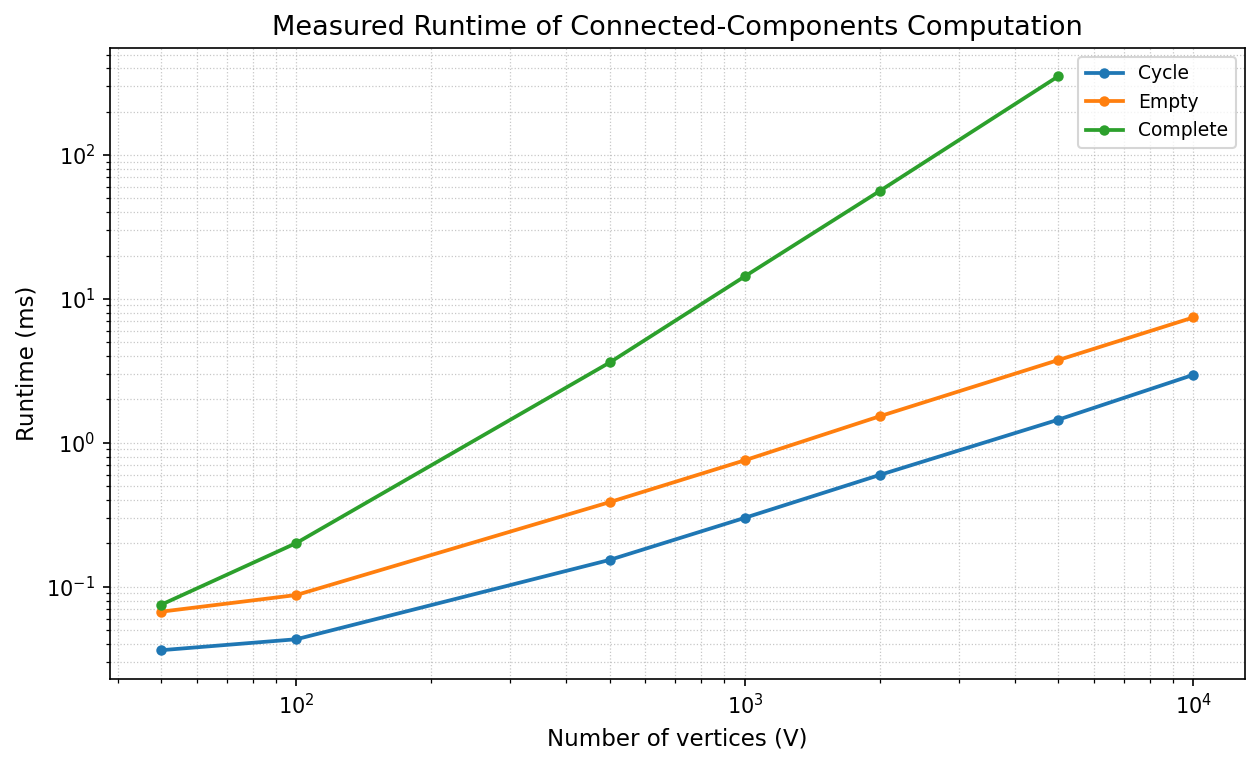
\includegraphics[width=0.82\textwidth]{figures/runtime_connected_components.png}
\caption{Measured runtime of connected-components computation.}
\end{figure}

\begin{figure}[ht]
\centering
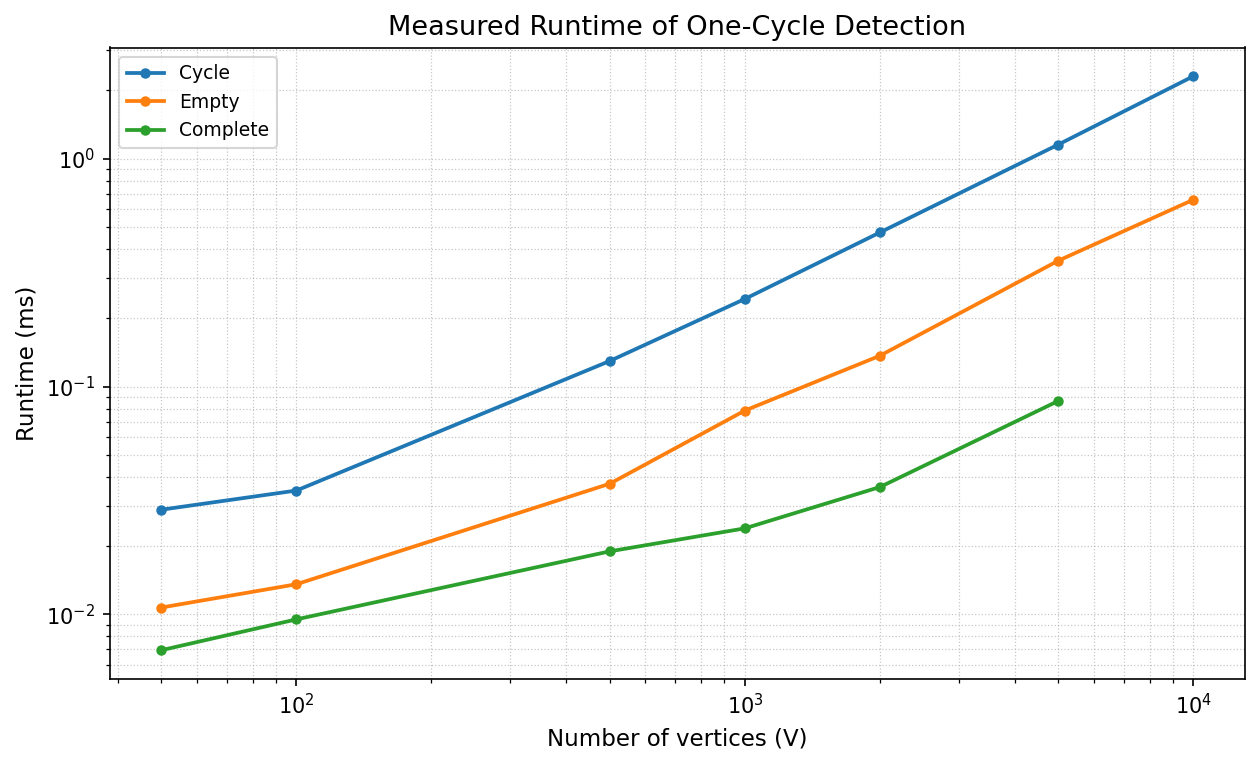
\includegraphics[width=0.82\textwidth]{figures/runtime_one_cycle.png}
\caption{Measured runtime of one-cycle detection.}
\end{figure}

\begin{figure}[ht]
\centering
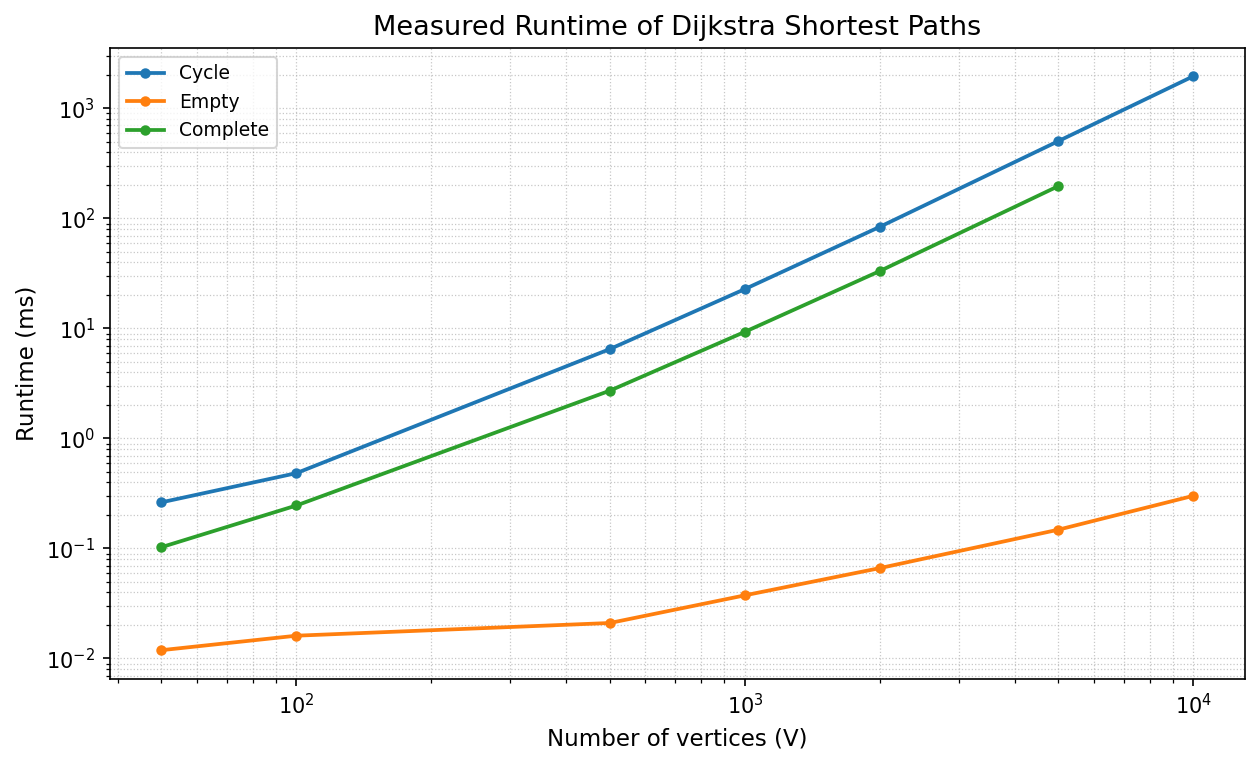
\includegraphics[width=0.82\textwidth]{figures/runtime_shortest_paths.png}
\caption{Measured runtime of Dijkstra shortest paths.}
\end{figure}

\clearpage
\subsection{Peak Memory}

Complete graphs show the largest process-level peak RSS because the adjacency
list stores every edge at both endpoints. At $V=5000$, the complete graph
contains 12,497,500 edges, with peak RSS of 164,512 KB for connected
components and 162,944 KB for shortest paths.

Cycle-graph shortest paths also show substantial memory growth: 2,496 KB at
$V=1000$, 6,064 KB at $V=2000$, 29,968 KB at $V=5000$, and 114,784 KB at
$V=10000$. The returned collection contains a full path for every reachable
destination, so output storage contributes to the measured memory.

\begin{figure}[ht]
\centering
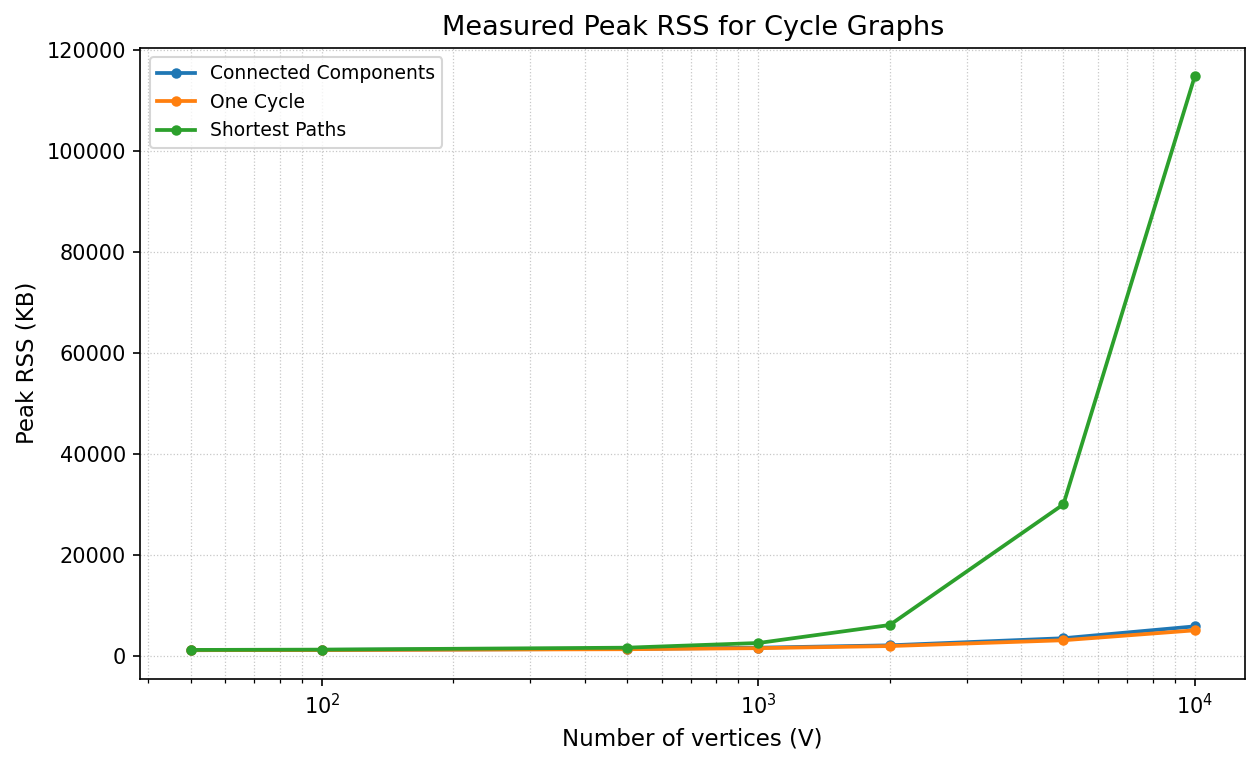
\includegraphics[width=0.82\textwidth]{figures/memory_cycle.png}
\caption{Measured peak RSS for cycle graphs.}
\end{figure}

\begin{figure}[ht]
\centering
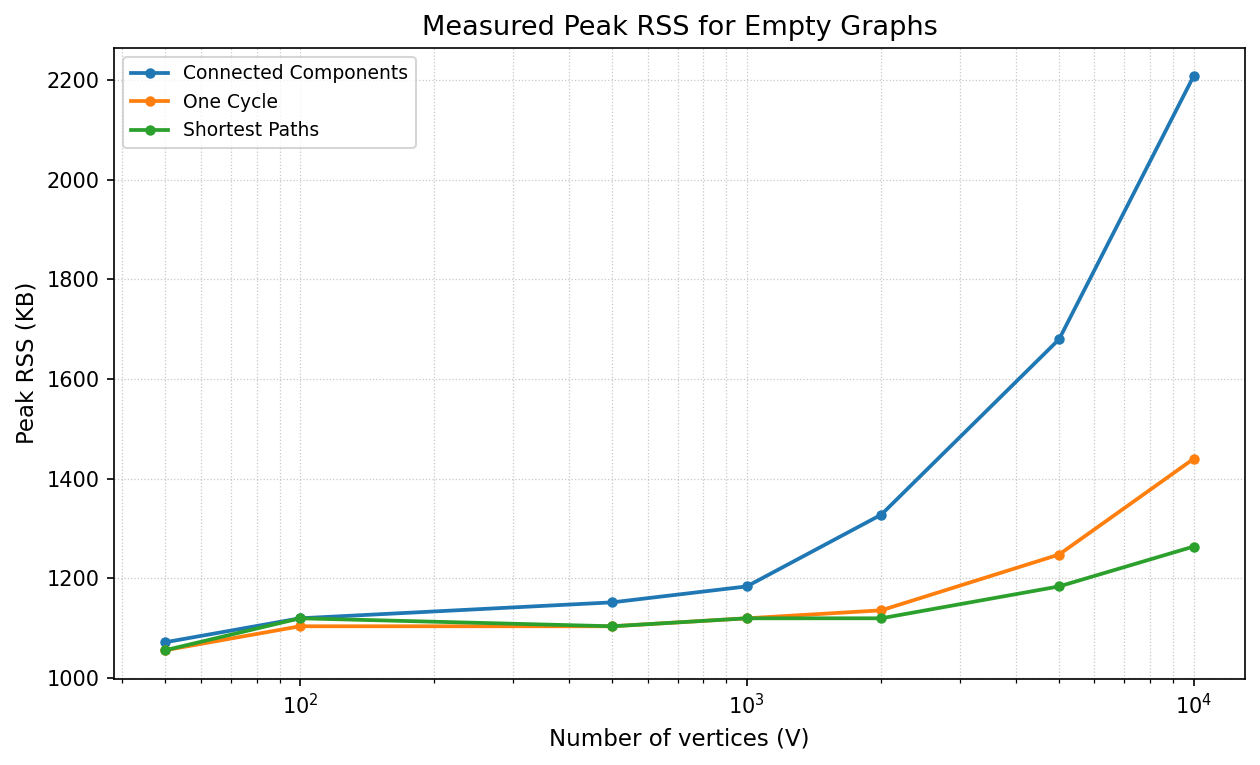
\includegraphics[width=0.82\textwidth]{figures/memory_empty.png}
\caption{Measured peak RSS for empty graphs.}
\end{figure}

\begin{figure}[ht]
\centering
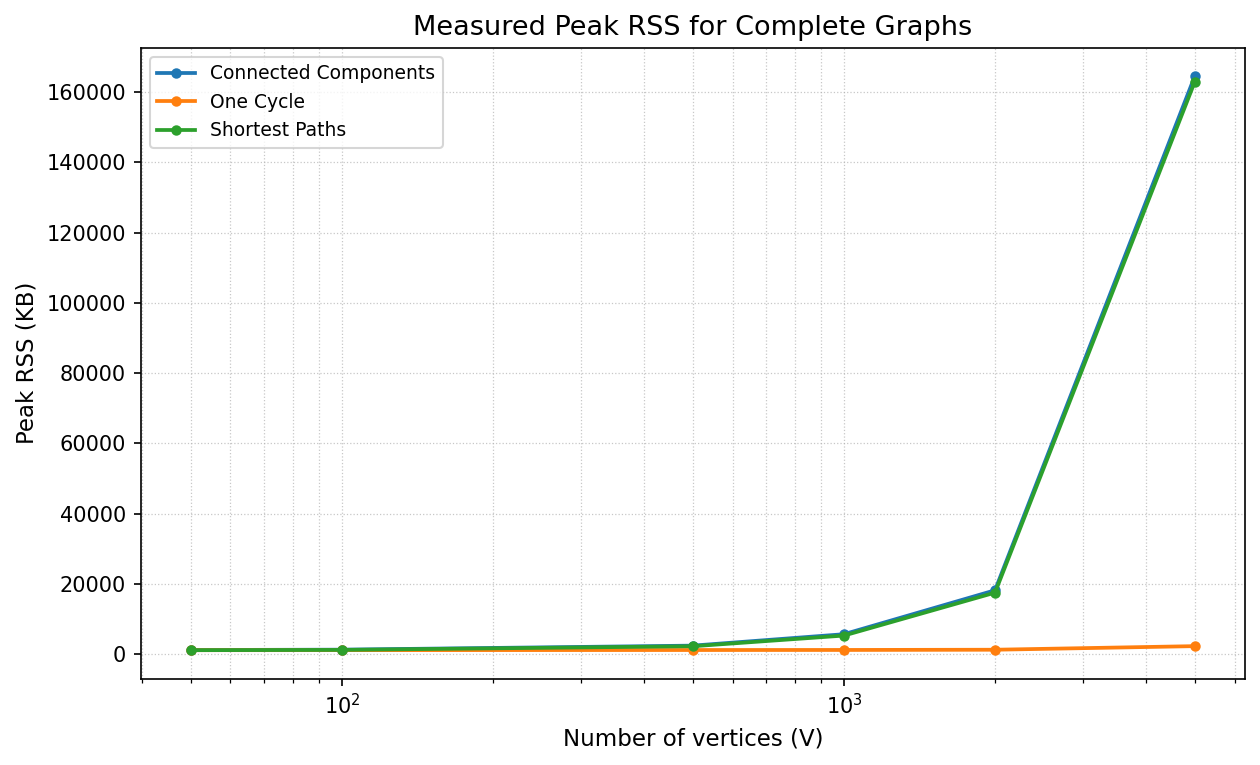
\includegraphics[width=0.82\textwidth]{figures/memory_complete.png}
\caption{Measured peak RSS for complete graphs.}
\end{figure}

\subsection{Overall Observation}

The experiments show that the number of vertices alone does not determine
performance. The number of edges, graph structure, early termination, and the
size of the required output all affect measured runtime and memory.

The observations are consistent with the theoretical complexity: sparse
graphs with $E=\Theta(V)$ scale differently from dense complete graphs with
$E=\Theta(V^2)$.

% ============================================================
\section{Conclusion}

The required graph algorithms were implemented using a custom undirected
adjacency-list representation in C++17. The implementation includes DFS
connected components, DFS-based one-cycle detection, and Dijkstra shortest
paths with implicit unit edge weights.

Three graph generators, correctness tests, and a runtime/peak-memory
experiment framework were also implemented. The final experiments cover
multiple graph sizes and both sparse and dense graph structures.

The measured results demonstrate the influence of $V$ and $E$ on
graph-algorithm performance while also showing practical effects of early
termination and shortest-path output size.


% ============================================================
% Real-world graph bonus
% ============================================================
\clearpage
\section{Optional Bonus: Real-World Graph}

\section{Bonus Objective}
The optional bonus extends the assignment from simulated graphs to a real-world graph with at least one million nodes. The required tasks are to identify and explain the data source, preprocess it into a usable graph representation, run the three graph operations, report runtime and peak memory, and evaluate at least three different adjacency criteria.

The purpose of this experiment is not to change the algorithms. Instead, it tests whether the same graph algorithms and implementation approach remain usable on a graph derived from a multi-million-node real dataset, and it shows how the definition of adjacency changes graph structure and measured behavior.

\section{Real-World Data Source}
The dataset selected was the \textbf{NASA HIRENASD coarse unstructured mesh}. NASA's Open Data Portal describes the dataset as an unstructured HIRENASD mesh with a coarse size of approximately 5.7 million nodes and 14.4 million elements, intended for node-centered solvers. The source page identifies the resource as \texttt{HIRENASD\_coarse\_nc} and provides a Tecplot ASCII resource named \texttt{HIRENASD\_coarse\_nc\_volume.dat.gz}. The NASA DASHlink resource identifies Markus Ritter as the contributing author and dates the resource to June 1, 2011.

\begin{itemize}
    \item NASA Open Data Portal: \url{https://data.nasa.gov/dataset/hirenasd-coarse-unstructured}
    \item NASA DASHlink resource: \url{https://c3.ndc.nasa.gov/dashlink/resources/382/}
    \item Direct Tecplot ASCII resource used: \url{https://c3.ndc.nasa.gov/dashlink/static/media/dataset/HIRENASD_coarse_nc_volume.dat.gz}
\end{itemize}

The NASA Open Data Portal does not specify a license for this dataset. Accordingly, the dataset is attributed to NASA/DASHlink in this report and is not presented as original data. The graph definitions, preprocessing methods, and measurements presented in this project were developed and obtained independently using the referenced source data.

\section{Preprocessing and Graph Representation}
The downloaded resource is a compressed Tecplot ASCII file. The preprocessing program reads the compressed stream without first creating a separate uncompressed one-gigabyte file. The mesh contains multiple volume and boundary zones with tetrahedral, pyramid, prism, triangular, and quadrilateral connectivity.

Node identifiers are local to zones, so preprocessing first maps coincident node coordinates to a single global vertex identifier. This produced \textbf{5,663,766 unique global graph vertices}. Undirected edges are then generated according to the selected adjacency criterion, duplicate undirected edges are removed, and the resulting graph is written as a compact CSR representation.

The CSR file contains a 32-bit vertex count, a 64-bit undirected edge count, a 64-bit offset array of length $V+1$, and 32-bit neighbor identifiers. The graph is therefore stored independently of the original Tecplot parser during algorithm execution.

\section{Adjacency Criteria}
Three graph interpretations were evaluated. These are modeling choices made for this bonus; the assignment requires three criteria.

\subsection{C1: Same-Element Adjacency}
Two distinct mesh nodes are adjacent when they occur in the same volume element. Each volume element therefore induces a clique on its distinct physical nodes. This creates the densest of the three graphs.

\subsection{C2: Mesh-Edge Adjacency}
Two nodes are adjacent only when they form a physical edge of the corresponding volume element. This is a more restrictive interpretation than same-element adjacency and is intended to represent mesh connectivity directly.

\subsection{C3: Boundary-Face Adjacency}
Two nodes are adjacent when they occur on the same boundary face. Triangular and quadrilateral boundary faces therefore create local face-based adjacency. This criterion does not connect the volume interior and consequently produces a much sparser graph.

\section{Preprocessing Measurements}
Table~\ref{tab:bonus-preprocessing} reports the measured preprocessing results. Peak memory is process-level maximum resident set size on the machine used for the experiment.

\begin{table}[H]
\centering
\caption{NASA HIRENASD preprocessing results.}
\label{tab:bonus-preprocessing}
\small
\begin{tabular}{lrrrr}
\toprule
Criterion & Vertices & Raw edges & Unique edges & Time (s)\\
\midrule
C1 Same-element & 5,663,766 & 171,626,243 & 53,425,834 & 53.95\\
C2 Mesh-edge & 5,663,766 & 114,700,195 & 24,939,650 & 50.11\\
C3 Boundary-face & 5,663,766 & 1,022,862 & 534,591 & 38.65\\
\bottomrule
\end{tabular}
\end{table}

The corresponding peak preprocessing RSS values were approximately 3.82 GiB for C1, 2.20 GiB for C2, and 522 MiB for C3. The differences are consistent with the different numbers of candidate and unique edges that must be accumulated during preprocessing.

\section{Algorithm Execution}
The three required graph operations were executed on each of the three graph representations. Runtime measures the algorithm execution after graph loading; graph construction is not included in the algorithm timing. Peak RSS is a process-level measurement and includes the graph representation inherited by the algorithm process, so it should not be interpreted as an exact allocation trace for the algorithm alone.

For Dijkstra's algorithm, every edge has implicit weight 1. The execution program selected a deterministic source vertex based on maximum graph degree and reported the selected source and degree. The same graph was used for all three algorithms under each adjacency criterion.

\begin{table}[H]
\centering
\caption{NASA HIRENASD algorithm execution results.}
\label{tab:bonus-execution}
\small
\begin{tabular}{llrrr}
\toprule
Criterion & Algorithm & Time (s) & Peak RSS (GiB) & Result summary\\
\midrule
C1 & Connected components & 0.345 & 0.494 & 1 component\\
C1 & One cycle & 0.004 & 0.049 & 4 cycle vertices\\
C1 & Dijkstra & 1.251 & 0.491 & 5,663,766 reachable; max dist. 65\\
\midrule
C2 & Connected components & 0.222 & 0.264 & 1 component\\
C2 & One cycle & 0.004 & 0.049 & 4 cycle vertices\\
C2 & Dijkstra & 1.206 & 0.277 & 5,663,766 reachable; max dist. 75\\
\midrule
C3 & Connected components & 0.034 & 0.053 & 5,493,288 components; largest 170,479\\
C3 & One cycle & 0.004 & 0.049 & 4 cycle vertices\\
C3 & Dijkstra & 0.037 & 0.090 & 170,479 reachable; max dist. 177\\
\bottomrule
\end{tabular}
\end{table}

\section{Validation and Evidence of Correct Execution}
The real-world experiment was checked at the graph-file and algorithm-output levels. The CSR loader verified the vertex count, edge count, offset-array length, monotonic offsets, final offset, neighbor count, and neighbor identifier ranges before running the algorithms.

For the measured runs, the connected-component results account for the complete graph vertex set: C1 and C2 each contain one component of all 5,663,766 vertices, while C3 reports 5,493,288 components with a largest component of 170,479 vertices. Dijkstra reports the number of reachable vertices and maximum shortest-path distance; its reachable count matches the full graph in C1 and C2 and matches the source component size in C3. Cycle detection returned a closed four-vertex representation in all three graphs, with the first and last reported vertex equal.

These checks provide experimental evidence that the algorithms operated on the intended graph representation. They are not a formal proof of implementation correctness; the formal correctness tests for the assignment are reported earlier in this report and produced ``All graph algorithm tests passed.''

\section{Comparison of the Three Adjacency Definitions}
All three graphs contain the same 5,663,766 global vertices, but the adjacency rule changes the number of edges and graph structure substantially.

\begin{table}[H]
\centering
\caption{Structural comparison of the three real-world graph definitions.}
\label{tab:bonus-comparison}
\small
\begin{tabular}{lrrrr}
\toprule
Criterion & Vertices & Edges & Components & Largest component\\
\midrule
C1 Same-element & 5,663,766 & 53,425,834 & 1 & 5,663,766\\
C2 Mesh-edge & 5,663,766 & 24,939,650 & 1 & 5,663,766\\
C3 Boundary-face & 5,663,766 & 534,591 & 5,493,288 & 170,479\\
\bottomrule
\end{tabular}
\end{table}

The experiment demonstrates that adjacency is a graph-modeling decision with direct algorithmic consequences. C1 creates the densest graph because every volume element induces all pairwise node connections. C2 has fewer edges but remains globally connected. C3 is much sparser and highly disconnected because it represents only boundary-face co-adjacency. Consequently, the number of reachable vertices and the measured execution cost of the algorithms change with the adjacency definition even though the underlying NASA dataset is unchanged.

\section{Bonus Observations}
\begin{itemize}
    \item The preprocessing stage is substantially more memory-intensive than the subsequent graph traversals because edge candidates must be accumulated and deduplicated before CSR output.
    \item Connected-components execution reflects graph size and edge count: C1 and C2 are both connected, while C3 contains many small components. For Dijkstra, the C3 source reaches only the 170,479-vertex source component.
    \item Dijkstra reaches all vertices in C1 and C2. Its maximum observed shortest-path distance is 65 for C1 and 75 for C2 from the selected source vertices.
    \item The C3 source component contains 170,479 vertices and has maximum reported distance 177. This value is a distance within the reachable component, not a distance over all 5,663,766 vertices.
    \item One-cycle detection is an early-terminating search. It found a valid cycle almost immediately in each dense graph, so its observed time is much smaller than a full $O(V+E)$ traversal even though the worst-case bound remains $O(V+E)$.
\end{itemize}

\section{Reproducibility and Source Attribution}
The bonus source tree includes the preprocessing and execution programs, the measured results, and documentation of the source dataset and adjacency definitions. The original NASA compressed dataset is not redistributed inside the submission because it is a large external source file; the documented NASA URLs allow the dataset to be obtained directly from the source. The generated graph binaries are also excluded from version control because they are large derived artifacts. The preprocessing program regenerates them from the documented NASA source.

\section{Bonus Deliverables}
The final submission includes the original required assignment materials together with the bonus preprocessing and execution source, bonus measurements, source attribution, and the combined report. The exact filenames \texttt{realgraph make.cpp} and \texttt{run realgraph make.cpp} are provided as the assignment's requested bonus entry points.

\end{document}
